\chapter{State of the Art}\label{chap:state-of-the-art}

A modular robotics is a way to build robots consisting of \emph{modules}. In
context of this paper, modules are rather high-level pieces with a certain level
of self-control instead of low-level components like individual actuators or
sensors. It might even make sense to talk about modules as individual robots,
which are used to build bigger robots. The modules have usually a limited set of
capabilities -- often the functionality is so primitive, the modules cannot
perform useful tasks on their own. However, when we join multiple modules, they
can cooperate and, therefore, new capabilities of the system as a whole emerge.
This idea probably first appeared in the work by
\textcite{DBLP:conf/icra/FukudaK90}, where they introduced CEBOTs (Cellular
Robotic System).

\section{Taxonomy of Existing Modular Robots}

Since the era of CEBOTs, many more projects followed and the research area split
into two: smart (or programmable) matter and modular robotics. The smart matter
aims at building very simple modules leveraging physical and chemical principles
(imagine artificial atoms) in order to create blob of modules, which can
reassemble into a different, usually solid, object based on an external input.
Contrary, the modular robotics aims at building more complex modules, which are
able of sophisticated self-organization (imagine artificial cells), which can
form usually highly dynamic robots that can autonomously move and interact with
their environment. Smart matter also aims at sub-millimeter modules, modular
robotics aims at sub-centimeter modules \cite{DBLP:conf/ieeealife/Christensen07,
1285597}. In the rest of this paper, we will omit smart matter and focus
exclusively on modular robots.

What distinguishes modular robots from swarm robotics is the ability of the
modules to mechanically connect and inherently form a larger robot. The
connection can be performed externally, e.g., by an operator, or the modules can
connect on their own. Even the trend is to build self-reconfigurable robots,
there are occasionally some exceptions, e.g., PetRo
\cite{DBLP:conf/ro-man/Salem14}.

There have been many more or less successful projects of self-reconfigurable
modular robots since the CEBOTs. The projects feature various designs approaches
from the capabilities of individual modules to the topology in which the modules
connect. Most of the projects used metamorphic modules, i.e., there is only a
single or a few types of modules in the system. We consider the following list
as a nice representable sample of the various designs: Fracta
\cite{DBLP:conf/icra/MurataKK94}, Molecule \cite{DBLP:conf/icra/KotayRVM98},
Polybot \cite{DBLP:conf/icra/YimDR00}, M-TRAN
\cite{DBLP:conf/icarcv/KurokawaKYTMK02}, Atron
\cite{DBLP:conf/iros/JorgensenOL04}, Superbot \cite{DBLP:conf/iros/SalemiMS06},
Molecube \cite{DBLP:journals/trob/ZykovMDL07}, Roombots
\cite{DBLP:conf/icra/SprowitzBDI09}, Symbricator
\cite{DBLP:journals/corr/abs-1109-2288}, SMORES \cite{DBLP:conf/iros/DaveyKY12},
M-Blocks \cite{DBLP:conf/iros/RomanishinGR13}, ModRED
\cite{DBLP:journals/ras/BacaHDND14}, HyMod \cite{DBLP:conf/dars/ParrottDG16} and
Omni-Pi-tent \cite{DBLP:conf/taros/PeckTT19}.

\textcite{4141032} distinguishes three categories of the robots based on the
topology in which they connect. Each category has its own specific problems of
control and makes some tasks easier than other:

\paragraph{Lattice architecture} have its modules arranged in regular 3D grid --
e.g., a cube or hexagonal grid. The modules are tightly packed together. Typical
examples of such architectures are M-Blocks \cite{DBLP:conf/iros/RomanishinGR13}
and Atron \cite{DBLP:conf/iros/JorgensenOL04}. The regular grid makes it easier
to create a reconfiguration schedule and execute in parallel (for more details
see Subsection \ref{sec:chal-reconfig}). However, reconfiguration is usually the
only option for locomotion of such system, and, therefore, lattice architectures
do not yield highly dynamic systems.

\paragraph{Chain architecture} have its modules connected in a string or
possibly in a tree. Typical examples of such architectures are Polybot
\cite{DBLP:conf/icra/YimDR00} and Molecubes
\cite{DBLP:journals/trob/ZykovMDL07}. This architecture allows for easy
formation of limbs and arms, therefore, these robots usually interact well with
the environment. Also even very simple controllers yield locomotion (via
snake-like movements (see Subsection \ref{sec:chal-locomotion} for more
details). The chains can also form space-filling curve, therefore, e.g.,
Molecubes, can form a lattice-like structures, while the underlying structure is
linear.

\paragraph{Hybrid architecture} allows for both arrangements of modules,
therefore combines the advantages of both, possibly at the cost of increased
complexity. Examples of such robots are M-TRAN~III
\cite{DBLP:journals/ijrr/KurokawaTKKHM08}, Roombots
\cite{DBLP:conf/icra/SprowitzBDI09}, SMORES \cite{DBLP:conf/iros/DaveyKY12},
HyMod \cite{DBLP:conf/dars/ParrottDG16} and Omni-Pi-tent
\cite{DBLP:conf/taros/PeckTT19}. We can perceive that the most recent trend is
to build hybrid architectures. Especially SMORES are designed to be able to
replicate arrangements of the other platforms, thus be as versatile as possible
\cite{DBLP:conf/iros/DaveyKY12}.

On top of the locomotion provided by the the inter-module interaction, some
systems feature locomotion of the individual modules - e.g, by providing wheels
(SMORES, HyMod) or tracks (Symbricator), which further makes the reconfiguration
problem easier by allowing the modules to move on their own in the space without
interaction with the rest of the modules. A good example of such solution is
work by \textcite{DBLP:journals/ral/LiuWY19}.

\section{Challenges of Modular Robots}

There are many common challenges of modular robotics and the robotics in
general. This challenges were nicely summarized recently in blog post by
\textcite{locklin_2020}. Most of the challenges can be characterized by shifting
the robots from single purpose devices used in industrial automation, which
follow a preprogrammed path ignoring any environment around them, to autonomous
devices which can move in and interact with environment and adapt to its
changes. The challenges includes problems like motion planning (how to get from
point A to point B and avoid obstacles), continuous mapping of the environment,
scene understanding, and affordance discovery (predicting how the object will
behave when the robot interacts with it).

In the rest of this paper, we will focus only on the challenges specific to
metamorphic robots. We will also deliberately omit the challenges of mechanical
and electrical design of such robots. We will only slightly touch them in
Section \ref{sec:mixed-challenges}.

Let us introduce the challenges and illustrate them on a simple case. Suppose
there is a robot composed out of the modules in a simple environment. See figure
\ref{fig:arena} for illustration of the environment. There are two elevated
ramps. On one of them, there is red cube. The robot is supposed to move the cube
from one ramp to another. There is also a power socket after a narrow passage.
The modules do not have enough energy to complete the whole task.

\begin{figure}[!t]
    \centering
    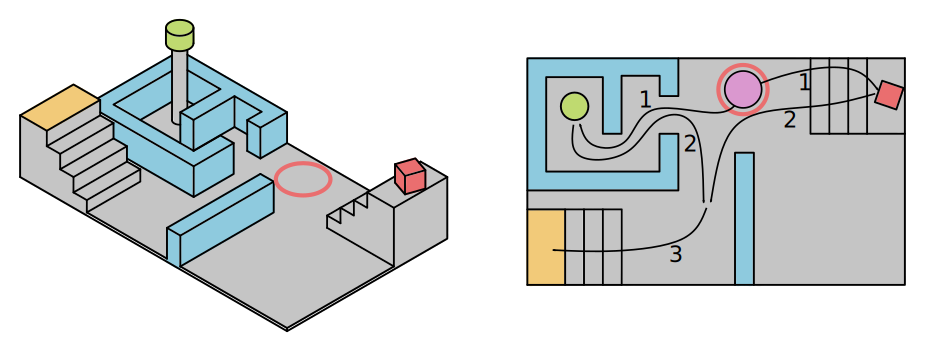
\includegraphics[width=0.7\textwidth]{figures/arena.jpg}
    \caption{The example environment for illustration of various challenges of
    self-reconfigurable robots.}
    \label{fig:arena}
\end{figure}

Once the robot is given the task, \footnote{Note, that for our purposes we omit
the translation step from "move the cube" to having a precise program saying
move to point A, grab a cube, move to point B, release the cube. We omit it as
we consider the translation as an open general problem of robotics.} we expect
it to find a plan to fullfil the task.

One of the possible solution is to first split in half and form two robots --
one will go to harvest energy, the second one will go and grab the cube. Then
then will join again on the way to the second ramp and share power. To do so,
the energy harvesting robot reconfigures into and energy efficient configuration
for locomotion and moves toward the narrow passage. Before the passage, it
reconfigure itself into a snake and passes it. Then it forms an arm and reaches
the power socket to charge itself. Meanwhile, the other robot moves towards the
first ramp. When it reaches the ramp, it changes shape so it can crawl the ramp
ramp and to grab the red cube cube. Then it returns and reunions with the energy
harvesting robot. They form a single robot and share the harvested power. During
climbing the other ramp, one of the modules in the systems stops responding,
therefore, however, the robot still continues to operate -- it just moves
slower. Before reaching the top of the ramp, the robots falls. It survives by
breaking inter-module connections to prevent module damage. The robots
reassembles and finishes the task.

Other possible solution (more suitable for cell-like robots, e.g., ATRON) is to
move in a \say{liquid blob of mass} which surrounds the cube and nudges it in
the desired direction.

In this simple example, we can identify several challenges typical for
self-reconfigurable robots. The first, obvious one, is \emph{planning
challenge}. The robot has to analyze the problem and figure out how to leverage
its ability to change shape to fulfill the task. The second challenge is the
challenge of \emph{locomotion} of the whole group of robots. Even the individual
modules can have wheels to move themselves, it is desirable to move in blocks as
new locomotion capabilities will emerge -- e.g. individual modules are not able
to climb stairs, but a system of them is. The next challenge is the
\emph{reconfiguration challenge}. This one is straightforward -- the robots have
to have an algorithm to compute reconfiguration plan to change shape. To
actually locomote, compute and schedule the reconfiguration we are facing the
\emph{control challenge}. We have to be able to control large number of modules
in a synchronized manner and ideally leverage all their computational potential.
All of the above should be designed in fault-tolerant way otherwise the large,
complex system will certainly fail. Also, the system has backed by solid
hardware and software solutions, which presents the \emph{mixed hardware and
software challenge}.

In the following section, we will discuss state-of-the-art for each of the
challenges individually.

\section{Planning Challenge}\label{sec:chal-planning}

For the purposes of this thesis, we consider planning for modular robots as an
effort to leverage the shape-changing ability of the self-reconfigurable robots
to fulfill tasks as efficient as possible and to adapt to an unknown or changing
environment. Note that planning often denotes also reconfiguration or locomotion
in the literature. For brevity, we also exclude work dealing with planning for a
single robot.

Despite we presented number of projects, nearly none of them deals with
planning. Instead, they focus rather on low-level control (locomotion and
reconfiguration), which we will cover in the later sections. To our knowledge,
there are two research groups that presented results in the area of high-level
planning of self-reconfigurable robots: SMORES and Symbricator.

There are several publications dealing with high-level planning for SMORES.
\textcite{DBLP:journals/arobots/JingTYK18} present a automata-based planner
(extension of their previous work \cite{DBLP:conf/ijcai/JingTYK17}), which takes
a task objective written in a \emph{Structured English}
\cite{DBLP:conf/iros/FinucaneJK10}. Their planner leverages a library of
handcrafted configurations. Each configuration have a set of properties and a
set of associated low-level controllers, which can perform single high-level
task -- e.g., move forward. The planner simply switches between those
configurations and controllers to achieve the specified goal. The switching is
based on a finite automaton. The automaton is synthesized from a set of formulas
in linear temporal logic (LTL) using an approach presented in
\cite{DBLP:journals/trob/Kress-GazitFP09}. The formulas come from the task
objective and additional constraints of the individual library configurations.
Note, that this approach is not brand new -- it was already introduced in
\cite{DBLP:conf/iros/CastroKK11} for CKBots, but work by
\textcite{DBLP:journals/arobots/JingTYK18} we just discussed, makes the approach
more robust and they present much more challenging experiments.

There is also work by \textcite{DBLP:conf/icra/TosunDJKCY18} on planning for
SMORES. They use a similar approach leveraging a library of hand-crafted
configuration as \cite{DBLP:journals/arobots/JingTYK18}. However, they extend
the system with \emph{environment augmentation modules} (just like
\cite{DBLP:conf/rss/PetersenNW11}) -- basically a passive modules serving as
building blocks for bridges and ramps, that can be used to augment the
environment, hence making fulfilling the objective easier for the robots.

Both of the presented approaches for SMORES use an external environment feedback
in the form of cameras with environment objects being tagged by black and white
patterns \cite{DBLP:journals/scirobotics/JingTYKC18}.

\textcite{DBLP:conf/syscon/LeviMRKVSLC14} take a different point of view on
planning for Symbricator. They focus and discuss mainly long-term plans for a
robotic system. Therefore, they propose that the planners should first focus on
the survival of the systems first (e.g., charging itself), and then, when
survival is guaranteed, the system should perform given tasks. Their
contribution lies in introduction of the \emph{SOS cycle}
(swarm-organism-swarm). In the cycle, the modules should first discover the
environment on their own (e.g., map it and locate power sources), then they
share the gathered information about environment. Then the modules assemble
together and fullfil a task. Once the task is completed (or failed), the modules
disassemble and the cycle repeats. In \cite{DBLP:conf/syscon/LeviMRKVSLC14},
they present advances on individual phases of the cycle (locomotion,
self-assembly, environment mapping). They also introduced concept of global
motion planning in \cite{DBLP:conf/icra/VonasekSKP13} using RRT
(rapidly-exploring random tree). This is an extension of the previous work
\cite{DBLP:conf/taros/VonasekKP12} by motion primitives -- a controllers for
specific configurations just like in the case of high-level planning for SMORES
\cite{DBLP:journals/arobots/JingTYK18}.

The current state-of-the-art in self-reconfigurable robot planning is making
progress, however, it is still far away from being applicable and, e.g.,
fulfilling the first grand challenge of modular robots
\cite{DBLP:journals/corr/abs-1108-5543}.

\section{Reconfiguration Challenge}\label{sec:chal-reconfig}

There is a variety of work dealing with the reconfiguration problem. The work
differs by problem specification, used approaches and a mathematical model of a
robotic system.

Most of the work considers reconfiguration from given initial configuration to
given target configuration on chain or hybrid module types. The expected output
of the reconfiguration is a sequence of connect/disconnect operations and joints
movements to perform in order to reach the target configuration. Since all the
movements take time to complete and consume energy, it is desirable to find the
shortest reconfiguration sequence. Also, it is highly beneficial if the
reconfiguration plan can be computed in distributed manner to leverage the
computation power of the individual modules.

Exploration of the state-space of the system is a straightforward approach.
However, as \textcite{DBLP:journals/jfr/ChirikjianPE96} showed, the number of
possible configurations grows exponentially, therefore, direct explorations is
infeasible even for small systems. \textcite{DBLP:conf/iros/Brandt06}
successfully applied RRT (rapidly-exploring random tree) for small systems of
ATRONs. \textcite{DBLP:conf/iros/AsadpourASI09} showed edit distance heuristics,
that can improve performance of the search and, therefore, increase size of the
configuration which is manageable by this approach. Similarly,
\textcite{DBLP:journals/ral/KhodrMHBI19} recently proposed some new pruning and
search heuristics. \textcite{DBLP:conf/monterey/BaarirHKR10} tackle the problem
of large state-spaces by using a symbolic representations inspired from software
model checking. All the work above demonstrates the results on MTRAN-like
modules.

Since the modules in a system are from the reconfiguration point of view
indistinguishable from each other, we should treat isomorphic configuration as
the same. There are some advances in this area leveraging specific properties of
the robotic systems presented in \textcite{DBLP:journals/ijrr/ParkCTY08},
\textcite{DBLP:conf/iros/AsadpourASI09} and
\textcite{DBLP:journals/ras/TaheriMAP16}.

One of the most interesting results in reconfiguration is done by
\textcite{DBLP:journals/ras/HouS14}. They introduce a model of robotic system
called a \emph{connector graph}). They show that the problem of finding the
shortest reconfiguration plan between two connector graphs is NP-complete. They
provide an exponential distributed algorithm and also an approximative
distributed algorithm running in polynomial time for the problem. Since
connector graphs capture only topology, this approach produces only
connect/disconnect actions. Hence, it might produce a plan which is not
collision-free and cannot be executed due to physical limitations. Such plans
are suitable for robots with good self locomotion (e.g., SMORES) but hard-to-use
in a system lacking individual modules locomotion (e.g., M-Blocks or M-TRAN).
When the modules can move on their own, they can simply disconnect from the
system, move to the target location, and connect there as presented in
\cite{DBLP:journals/ral/LiuWY19}.

As the reconfiguration on connector graphs is NP-complete,
\textcite{DBLP:journals/pcs/GorbenkoP12} present a solution to the
reconfiguration via reduction to the Boolean satisfiability problem (SAT).

Other results aim at finding a feasible plan rather than the shortest one. To
name a few, \textcite{10.1117/12.360345} use the divide and conquer approach.
\textcite{DBLP:conf/icra/HouS08} present a reconfiguration emerging from local
behaviors in tree configurations. \textcite{DBLP:journals/ral/LiuWY19} use
dynamic programming for reconfiguration between tree configurations.

\textcite{DBLP:conf/iros/ButlerBR01} present a \emph{Pac Man} algorithm for
transportation of modules on the 2D perimeter of a lattice robot with cube
modules. This algorithm is a base for naive reconfiguration -- by simply sending
one module by one to the goal destination. The Pac Man algorithm was extended to
3D surface a year later in \cite{DBLP:conf/wafr/ButlerR02}.
\textcite{DBLP:journals/dc/WalterWA00} gives a distributed algorithm, which is
however incomplete -- there exists configurations between it is not able to find
reconfiguration path. \textcite{DBLP:conf/icra/VassilvitskiiYS02} present a more
efficient distributed algorithm for reconfiguration of lattice type robots,
which is complete with only one restriction: they use $2\times2\times2$
meta-modules for the reconfiguration. The initial and target configurations have
to overlap at least on one meta-module.
\textcite{DBLP:conf/ieeealife/Christensen07} adapt similar approaches for
ATRONs. They use meta-module composed out of three modules. They compute
reachable positions on the surface of a blob of modules and then move the
meta-module along the shortest path on the surface. They can also move multiple
modules in parallel. Later, \textcite{DBLP:journals/comgeo/AloupisBDDFIW13}
presented asymptotically better algorithms for reconfiguration of lattice type
robots using non-uniform meta-modules. Additionally,
\textcite{DBLP:conf/pdp/PirandaB16} present a distributed rule-based algorithm
for reconfiguration of lattice type robots.

When reconfiguration using a distributed algorithm emerges from local behaviors,
an essential part of the whole process is detection if the target configuration
was reached. \textcite{DBLP:conf/icra/ButlerFRW02} present a distributed
algorithm for the problem. The algorithm assume only the neighboring modules can
excahnge messages. The algorithm runs in $\mathcal{O}(n^2)$ time. Later
\textcite{DBLP:journals/ras/BacaWDN17} present another algorithm, which expects
the modules in the configuration can communicate via broadcast (i.e., wireless
communication).

The approaches presented above yield deterministic reconfiguration plan.
\textcite{4141032} appeled that stochastic reconfiguration approaches should be
applied to modular self-reconfigurable robots. To our knowledge, to date
stochastic reconfiguration is widely used for smart-mattery and similar
minimalistic modular robots (e.g., Catoms \cite{DBLP:conf/aaai/KirbyCAPHMG05})
but have not been widely adapted for \say{full-featured} modular robots we are
interested in in this paper.

Overall, we can see that many approaches have been used to tackle the
reconfiguration problem and several solid theoretical findings have been made.
Though, we can still find open subproblems in this area. All the solutions
presented above assume there are no environmental effects (e.g., gravity) and
modules' joints have unlimited strength. \textcite{DBLP:journals/jr/SuzukiIKK11}
present an algorithm to augment existing configuration to minimize mechanical
stress. However, their work is not focused on reconfiguration between arbitrary
configurations.

In practice, the joints have limited strength and, e.g., the lattice structures
do not match perfectly. This is discussed in quite recent work by
\textcite{DBLP:journals/ras/HauserMLKBI20}, where they present an experiment in
which 12 Roombots assemble themselves into a chair.

Similarly, nearly none of the work deals with dynamics of the reconfiguration.
\textcite{DBLP:conf/iros/RomanishinMR19} partially deals with the dynamics in
the reconfiguration as M-Blocks rely on dynamic movements (caused by braking of
fast spinning flywheel) to reconfigure.

Also, there is no known approach of computing a collision-free reconfiguration
plan for chain and hybrid robots in distributed manner directly on the modules
using their computation power. Therefore, we can see a recent trend in the
reconfiguration: the target has shifted from finding the optimal reconfiguration
plan to finding a feasible reconfiguration plan (possibly working only on a
class of configurations), which can be computed more cheaply, possibly with
online updates.

\section{Locomotion Challenge}\label{sec:chal-locomotion}

The modules in self-reconfigurable systems are usually intentionally designed
with limited set of capabilities and it is expected that new capabilities emerge
when multiple modules join. Therefore, the modules often have no dedicated
actuator for locomotion. Having no dedicated actuators makes the modules simpler
and more suitable for usage as building blocks for larger robots, however, it
presents an additional challenge of locomotion of individual modules and blobs
of modules. Once a controller for locomotion is found, it can be used a motion
primitive for planning as we showed in Section \ref{sec:chal-planning}.

SMORES \cite{DBLP:conf/iros/DaveyKY12}, HyMod \cite{DBLP:conf/dars/ParrottDG16}
and Omni-Pi-tent \cite{DBLP:conf/taros/PeckTT19} face the challenge of lomotion
of individual modules by clever hardware design. Their modules do not have
dedicated wheels, however, they have wheels attached to one of the robots joint.
Such solutions allows for easy movement of individual modules (often referred as
\emph{micro-locmotion} in literature). Similarly, Roombots
\cite{DBLP:conf/icra/SprowitzBDI09} can use part of their module's hull as a
wheel. M-Blocks do not have wheels, but the can jump and shoot themselves into a
desired direction as a form of micro-locomotion
\cite{DBLP:conf/icra/RomanishinGCR15}.

Lattice type modules are designed to fit a grid, therefore, they often have no
body features which could serve a limb for movement, and, also they have modules
without any joints (e.g., M-Blocks). Therefore, their modules cannot locomote on
their own and can only move via reconfiguration \cite{1285597}. Such motion
often resemble fluid flow. This was first demonstrated by
\textcite{DBLP:conf/iros/YoshidaMKTKK01} on MTRANs. The authors manually created
a locomotion plan for a thick bar of modules, where modules from the end of the
bar crawl to the front. This procedure repeats and yields locomotion of the bar.
The previous approach was further generalized by
\textcite{DBLP:conf/icra/ButlerKRT02}.
\textcite{DBLP:conf/ieeealife/Christensen07} present a locomotion based on
reconfigurations for ATRONs. Their meta-modules can crawl on the surface of
existing robot. Similarly as in the case of M-TRANs, the modules from back move
to front. However, unlike M-TRANs, this procedure is fully automatic and has no
hand-crafted gaits.

Chain and hybrid type modules have several degrees of freedom, thus they can use
part of their bodies or other modules as limbs and form snake-like
\cite{DBLP:conf/icra/YimDR00, DBLP:conf/iros/KamimuraMYKTK01,
DBLP:journals/ijrr/KurokawaTKKHM08, DBLP:journals/arobots/JingTYK18}, crawl-like
\cite{DBLP:conf/icra/YimDR00, DBLP:conf/iros/KamimuraMYKTK01,
DBLP:journals/ijrr/KurokawaTKKHM08, DBLP:journals/arobots/JingTYK18}, walker
\cite{DBLP:conf/iros/KamimuraMYKTK01, DBLP:journals/ijrr/KurokawaTKKHM08,
mtranwalker} or rolling motion \cite{DBLP:journals/ijrr/KurokawaTKKHM08,
DBLP:journals/ijrr/SastraCY09, DBLP:journals/arobots/JingTYK18}. Furthermore,
\cite{DBLP:conf/iros/YimSSPDT07a} and \cite{DBLP:journals/ijrr/KurokawaTKKHM08}
show simple crawling of either individual module or pairs of modules in the free
space.

Practically all platforms presented so far have a list of hand-crafted
primitives for such motions. \textcite{DBLP:conf/isrr/TosunJKY15} present a tool
to aid hand-crafting of controllers for locomotion. The tools allow for
decomposing the controllers and turning them into library. It also gives means
to validate the designed controller. Despite that, the hand-crafted locomotion
plans do not scale well, thus automatic generation of them or omitting them
completely is desireable.

One approach for automatic generating locomotion plans is to use state-space
search similarly like in the case of reconfiguration.
\textcite{DBLP:conf/robotik/BonardiMSVI12} show this procedure using D*
algorithm for locomotion of individual module in a space filled with passive
mounting points. Such approach makes sense for Roombots as it is hard to
manually create motion primitives due to the non-orthogonal arrangements of
their axes. \textcite{DBLP:conf/dars/YoshidaKKMTK04} create locomotion and
motion plans for M-TRANs using RRT. Similar approach was later used by
\textcite{DBLP:conf/taros/VonasekKP12} for Symbricator.

Another approach is to apply machine learning for finding suitable locomotion
controllers. \textcite{DBLP:conf/eh/BennettR00} use genetic programming for
controller synthesis for 2D lattice-type robots. The controller is supposed to
find a path through narrow passage. The authors design a simple language for the
robots and perform mutations over it. Roombots also used genetic programming for
finding locomotion gaits in free environment \cite{aydn_2010,
DBLP:journals/procedia/PouyaAMI11}. \textcite{DBLP:journals/ras/ChristensenSS13}
present a distributed learning approach to generate locomotion for ATRONs. In
their setup, all modules run the same controller and based on externally
received reword, they adapt. Furthermore, \textcite{DBLP:conf/iros/DuttaDN17}
apply game theory to synthesize crawl-like gait for chain robots.

\textcite{DBLP:conf/icra/LipsonP00} proposed rather utopic idea for machine
learning on self-reconfigurable robots. They propose not to only apply machine
learning to the controllers, but also apply it to the mechanical design of the
modules itself and procude quick prototypes using 3D printers. After 20 years
from the publication, the technogy advanced a lot, however, we are not aware of
anyone trying to apply this approach in practice.

Instead of predefined motions it is also possible to use emerging behavior of
simple controllers of the modules. This approach often yields snake-like or
caterpilar-like motions. This was demonstrated by \textcite{stoy2002global}
further extended by them in \cite{DBLP:conf/icra/StoySW03}. The same authors
also present an approach where they use identicall controllers which can switch
roles during runtime in \cite{1159219} to produce locomotion.
\textcite{gonzalez2006locomotion} present new types of locomotion based on
sinusoidal patterns. Such solution scales well as the controllers are simple
and independent. However, the pallette of such motions is limited. The following
work mostly deals with execution and synchronization of such controllers, which
we will discuss more in depth in the following Section \ref{sec:chal-control}.

\todo{Rework the previous paragraph and distinguish Phase automata and CPG?}

Overall, the area of locomotion for self-reconfigurable robots is well explored
and there are approaches to tackle the specifics of self-reconfigurable robots.
However, this problem shares common open problems with general robotics like
execution locomotion plans on physicals robots in real environment, where the
robot has a limited knowledge of the enviroment based on sensors.

\section{Control Challenge}\label{sec:chal-control}

In the previous sections we discussed planning, reconfiguration and locomotion
of the self-reconfigurable robots. The presented approaches give its output in
the form of algorithms, plans, automata and more. For purposes of this paper, we
mean by \emph{controlling} a robot an application of the former results. Note
that in literature, the terms \emph{controlling} or \emph{controller} are often
used in a wider meaning -- it covers reconfiguration, planning or locomoton. The
application presents new challenges in the context of self-reconfigurable
robots. The robots present a distributed system, therefore the challenges
include problems of communication, synchronization and scalability of such
solutions. Note that in the following text, we will focus mainly of specifics to
robotic environment and omit general problems of distributed computing.

The existing robotic systems use various means of communication, which states
different requirements for the control approaches. These include two basic
types:

\paragraph{Broadcast and bus communcation} can be realized either
wirelessly over radio waves (e.g., WiFi in the case of
SMORES~\cite{DBLP:conf/iros/DaveyKY12}) or over a bus spanning thoughout the
whole robotic system (e.g., CAN in the case of
HyMod~\cite{DBLP:conf/dars/ParrottDG16}). Both of these types allow for simple
broadcast, thus distribution of information and synchronization is trivial.

However, both bus and wireless communication present a technical challenge.
Widely used technologies like WiFi, Bluetooth or ZigBee are not designed for
hundereds, possibly thousads, of agents spatialy placed near each other -- the
shared medium will congest. The bus communication has the same limitation. Also,
high-speed buses spanning through large robots present a challenge from
technical point of view (parasitic inductance of the traces, impedance
matching)~\cite{DBLP:conf/dars/ParrottDG16}.

Nevertheless, wireless communication gives the ability for disconnected parts of
the system to communicate. \textcite{DBLP:conf/iros/YimSSPDT07a} and
\textcite{DBLP:journals/corr/abs-1109-2288} cleverly use IR transceivers not
only to communicate between disjoint parts of the system, but also for
localization and navigation.

\paragraph{Point-to-point and hierarchical communcation} addresses the problem
of shared medium by having a communcation link only between negihboring modules
via connectors and thus, having separate medium between each pair of neighboring
modules. Such solutions scale well, however, the modules need to be able to
route the packets if module-to-module communication or broadcast is required.
The routing increases latency of the communication and brings extra complexity
to the module design.

The module-to-module connection is often realized via IR transceivers as it can
be also used for connector alignment and navigation.
\cite{DBLP:conf/iros/YimSSPDT07a}. \textcite{DBLP:journals/corr/abs-1109-2288}
cleverly use traditional Ethernet for communication between the Symbricator
modules, which provides robust and fast connection lines. The routing is
offloaded to Ethernet-switch ICs (therefore, does not introduce extra complexity
to the modules).

\bigskip

When broadcast communcation is available, the simplest approach is to use
central control either in the form of external entity (a server) or in the form
of single master module. The master can run centralized algorithm and provides
synchronization. Having a master, however, kills one of the appealing feature of
the system -- it presents a single point of failure thus limits fault-tolerance.
Also, the single master limits scalability of the system. The master can be
authomatically elected by one of well known algorithms for leader election in
distributed systems \cite{baca2016coordination}, thus mitigate the problem of
single point of failure. Nevertheless, central control is widely used for
protyping: e.g., \cite{DBLP:journals/ijrr/KurokawaTKKHM08,
DBLP:conf/icra/TosunDJKCY18} use external control entity for experiments and
\cite{superbotroller} use a master module.

Therefore, the general aim is to introduce distributed solutions. We can find
general solutions providing frameworks for distributed control in the
literature, however, they are often either orientated on industrial automation
or too heavy to deploy on simple modules. The popular Robotic Operating System
\cite{DBLP:journals/corr/abs-1809-02595}, which aims for distributed real-time
control, is usually consedered heavy, and thus the researchers look for more
lighweit solutions for self-reconfigurable robots.

Global synchronization among the modules in a systems allows to apply many
traditional controllers formalisms including gait tables
\cite{DBLP:conf/icarcv/KurokawaKYTMK02, DBLP:conf/iros/YimSSPDT07a},
automata-based controllers \cite{DBLP:journals/procedia/PouyaAMI11,
DBLP:journals/arobots/JingTYK18}, nested-controllers \cite{1159219} and more.

We can find multiple solutions to the synchronization.
\textcite{DBLP:journals/ijrr/ParkCTY08} use \emph{robotic bus} \cite{roboticbus}
for synchronization. The synchronization is as essential part of the bus.
\textcite{yim1994locomotion} proposes that each module should be equipped with
internall clocks and they are occasionally synchronized among the modules. When
an action should start, the start signal is equipped with a timestamp in the
future when the action should start, so the broadcasting can complete in time.
\textcite{stoy2002global} present a synchronization algorithm for periodic
actions. The algorithm is roubus to loss of synchronization signals and the
number of modules.

Digital hormones present a biologically inspired approach to control, which can
be agnostic of the number of modules in the system and communication faults. It
also scales well. Digital hormones concept was probably first introduced by
\textcite{DBLP:conf/agents/ShenLW00} and more extensions followed
\cite{DBLP:conf/icra/SalemiSW01, DBLP:journals/trob/ShenSW02}. In a nutshell,
digital hormones are messages passed between the robots just like the biologial
ones. When a module receives a hormone, it can trigger various action. Also, the
module can detect number of received hormones and send hormones to its
neighbors. Hormone control is suitable for robots featuring point-to-point
communication as it requires no routing (the hormone rules define the routing
implicitly). \textcite{DBLP:conf/cec/HamannSSC10} introduced \emph{artificial
homeostatic hormone system}, which allows for \say{infusion} of hormones inside
the robot body, thus controlling it. This system is able of
self-synchronization, which has proven to be roubust.
\textcite{DBLP:conf/icra/MorenoG11} combined hormone-based approach with central
pattern generators to achieve locomotion of chain type robots. The hormones
carry feedback information from the sensors.

Altough the hormone based approach seems to be promising, so far only a limited
set of tasks was accomplished using it. Instead, we see that most of the work
deals with traditional controllers supported by global synchronization.

\section{Fault-tolerance Challenge}

There is no single widely accepted interpretation of what fault tolerant systems
should comply to. Usually, in a context of embedded system, a system is
considered fault-tolerant when it is able to continue operating (possibly with
worse performance) after one of its components fails
\cite{DBLP:journals/micro/Johnson84}. The extent of fault-tolerance depends on
what type of failures the system survives.

For example, we usually consider living organisms as highly fault-tolerant
systems. If an animal looses an limb, it is able to adapt and perform similar
tasks. E.g., a cat without a leg is still able to move and climb -- possibly
slower, but it is able to survive. As we outline in the beginning of this
chapter, the ability to build fault-tolerant robots is highly desirable and
building self-reconfigurable metamorphic robots can be a viable way.

We already presented several solutions to planning, locomotion and control of
such robots and we briefly outlined their robustness to faults. In the rest of
this section, we provide another view on fault-tolerance; we will look on
various types of faults in modular system and recap state-of-the-art for them.

\cite{DKbotDistr} and \cite{4141032} discuss several aspects of
fault-tolerance. We can distinguish several types of fault:

\paragraph{Complete module malfunction,} where the module stops responding and
acts passively. The usual assumption is that the other modules in the system can
detect such module. This type of malfunction is probably the most mentioned one
in literature. The usual solution is to either drop or to ignore such
modules and reconfigure into a new configuration
\cite{DMotionCoord, DBLP:conf/ieeealife/Christensen07, DBLP:conf/iros/DaveyKY12}.

\paragraph{Byzantine module malfunction,} where it is not easy to detect the
module has failed -- e.g., the module can have a faulty sensor so it will report
wrong data to other modules. The module can even be malicious. There is not much
work on this type of malfunction in the context of metamorphic robots as far as
we are aware. However, in context of distributed systems and sensor networks in
general, it is a vivid research topic.

\paragraph{Actuator malfunction,} where the module control unit is fully
functional, however, one or more of the modules actuators are either stuck
in a position or spin freely. This type of malfunction was tackled by
\textcite{DBLP:conf/romoco/VonasekONW15}.

\paragraph{Explosion of the whole system} is a type of malfunction where the
robot is broken down into pieces randomly spattered over the environment usually
after a high energy impact. \textcite{DBLP:conf/iros/YimSSPDT07a} proposed a
solution for automatic reassembly after explosion. They also discuss, that
system explosion is a way of fault-avoidance. When a system can reassemble, it
is desirable to include weak, re-attachable joints, which protect the individual
modules.

\section{Real-world Challenges}\label{sec:mixed-challenges}

So far, we focused on the theoretical challenges of the self-reconfigurable
robots. However, to validate the theory and to make these robots practical, we
have to also tackle the practical, more engineering challenges.

The first and the most obvious one is the challenge of hardware miniaturization.
Various researches claim, that we should build target at roughly 1cm modules
\cite{1285597, DBLP:conf/ieeealife/Christensen07}. Otherwise, we will not be
able to build complex enough and small enough robots out of them. Contrary to
that, the authors of Roombots suggest to build larger robots, around 10~cm, to
make them strong and powerfull enough to interact with everday objects
\cite{DBLP:conf/icra/SprowitzBDI09}. Most of today modules fits to size around
10 cm (e.g., Roombots, SMORES) or 6 cm (e.g., M-Blocks, Molecubes). The smallest
module so far are Femtobots \cite{Femtobots} with size less than 1~mm. However,
these modules are rather suitable for smart-matter due to their limited
capabilities.

Directily with the hardware miniaturization comes the challengeof connecting the
modules via connectors. Connectors are the essential part of the robots. They
have to be strong enough to support large robotic structures and small enough to
fit inside the module. Basically every platform we introduced so far comes with
its custom connector. We currently conside the SMORES's EP-FACE
\cite{DBLP:conf/iros/TosunDLY16}, HyGen \cite{DBLP:conf/iros/ParrottDG14} and
our RoFICoM \cite{DBLP:conf/iros/MrazekB19} as the most advance connectors for
self-reconfigurable robots so far.

In addition to miniaturization cames the question, whether the current advances
in control can be applied to physical robots due to the limited computation
power. \textcite{DBLP:journals/ral/Trenkwalder19} discusses the computation
power of recently released miniature robots and gives nice overview on what can
and what cannot be computed on the robots. Currently, the algorithms allowing
for interaction with the environment, such as computer-vision and continuous
environment mapping, are practically impossible to compute on miniature robots.

If we ever deploy self-reconfigurable robots to the real-world, we will also
have to tackle the question of security. \textcite{DBLP:conf/icas/HigginsTM09}
rais question about security of swarm robots and discusses what types of
attack could be performed on such robots. In our opinion the same applies to
modular self-reconfigurable robots. There is no active research in this are as
far as we are aware -- probably this area is far away from being applied to
practice to raise these questions.

Currently, many of the challenges we can solve individually. However, we still
lack a single \say{full-featured} self-reconfigurable platform, which would
solve most of the problems simullteanously.

\section{Reproducibility of Results}\label{sec:reproducibility}

As we have briefly outlinen in Chapter \ref{chap:introduciton}, we percieve the
advance in this field quite splattered and incoherent due to lack of proper
reproducibility. The theoretical paper we encountered gives proofs of their
claims, thus we can consider them as reproducible. However, papers providing
sophisticated software solutions often lack public implementation. Thus, that
are outside the original team of authors cannot build on top existing results.

Similarly, when papers introduce hardware solutions, e.g., in the form of
robotic platforms, they do not provide technical documentation, CAD models or
bill of materials. This is even the case of papers which contribution is the
design of an easy-to-build and low cost robots \cite{DBLP:conf/robio/YuLW17}. We
also contacted autohors of several platforms. The usual response was that the
designs are not worth publishing (due to poor organization and missing
structure), the authors did not thought about publishing them or the designs are
confidentia. To our knowledge, the only exception is the project Dtto
\cite{otrebla333} and the project Symbricator
\cite{DBLP:journals/corr/abs-1109-2288}, where we were able to dig some
technical specification in the form of master thesis in archives. However,
proper central resource is missing.